% {{{ Preamble
\documentclass[pdftex,12pt,a4papaer]{report}
\usepackage[pdftex]{graphicx}
\usepackage{fancyhdr}
\usepackage{parskip}
\usepackage[numbers]{natbib}
\usepackage{url}
\usepackage{amsmath}
\usepackage{amsfonts}
\usepackage{setspace}
\usepackage{paralist}
\usepackage[]{units}
\usepackage{tabto}
\usepackage{float}
\usepackage{comment}
\usepackage{titling}
\usepackage{hyperref}
\usepackage{todonotes}
\usepackage{textcomp}
% \usepackage{minted}
\pagestyle{fancy}
% }}}
\setlength{\marginparwidth}{3cm}

\linespread{1.5}

\title{DRACL 2.0 Proposal}
\author{Steven Allen}
\date{\today}

% {{{ Header
\rhead{\thedate}
\chead{\thetitle}
\lhead{\theauthor}
% }}}

\newcommand{\note}[1]{\textit{\textbf{Note:} #1}}

\begin{document}

\thispagestyle{plain}

\begin{center}
    \vspace*{\fill}
    {%
        \onehalfspacing{} \bfseries \Large
        DRACL (Decentralized Resource Access Control List) \\
    }

    \vspace{\fill}
    {\large
    \begin{minipage}{0.9\textwidth}
        \emph{Author:} \theauthor{} \hfill \emph{Advisor:} David Karger
        \\
        \begin{center}
              \thedate{}
        \end{center}
    \end{minipage}
    }
    \vspace*{\fill}
\end{center}

\tableofcontents

\newpage

\chapter{Introduction} 

DRACL is a decentralized, privacy-preserving access control system that allows
users (content owners) to control access to content hosted on services (content
hosts) by providing these services with access control lists (ACLs) that specify
which users and groups that should be granted access.

% TODO: Not quite correct. ACLs are private...

\section{Terms}

For convenience, we define the following terms:

\begin{compactdesc}
    \item[User] An end user.
    \item[Identity] An assumed identity. That is, identities may not correspond
      one-to-one to real people. They may be pseudonymous, or may correspond to
      a group or people.
    \item[Content Owner] A user that publishes content and wishes to control
      access to said content.
    \item[Consumer] A user that accesses content published by a content owner
      with the owner's permission.
    \item[Authorized Consumer] A consumer that is authorized to access a
      particular resource.
    \item[Group] A group of users as defined a content owner. In DRACL, groups
      are the unit of access control (i.e., content owners grant access to
      groups, not directly to individual consumers).
    \item[Authentication Provider] (AP) A service for facilitating
      authentication. Every DRACL user will have an AP (just like every email
      user has an email provider). Basically, the AP can perform limited
      actions on behalf of users while offline and can help ensure that a
      compromise of a user's account is recoverable.
    \item[Content Host] A party using this system to authenticate content it
      hosts. For example, Flicker, Facebook, Imgur, etc.
\end{compactdesc}

\section{Goals}

DRACL aims to provide a practical, secure, privacy preserving, and developer and user
friendly access control system.

By practical, we mean that DRACL should be designed to work in the world as it
is, not as we wish it were. For example, it shouldn't assume that users will run
their own servers or pay for anything for that matter, that content hosts will
invest a significant amount of time or resources in adapting their systems to
work with DRACL, or that some benevolent universally trusted third party will
pay for an oracle server capable of answering access control requests on-demand
in real time. This means that any third party servers that DRACL requires must
be low cost and at most semi-trusted and and can be expected to be, at best,
semi-reliable.

By secure, we mean that content owners should be able to efficiently revoke
access from consumers, compromises of content owner accounts should be
recoverable, and only authorized consumers should be able to access content.
Importantly, there should be no trusted third party that can act on behalf of
its users.

By privacy preserving we mean that DRACL should (1) not reveal the social
networks of its users to any party and that DRACL should (2) not reveal the
identity of consumers to content hosts. Unfortunately, this goal isn't entirely
achievable in a practical system but DRACL gets pretty close.

Three explicit non-goals of DRACL are:

\begin{enumerate}
\item Hiding the identities of content owners (anonymous publishing).
\item Hiding content from content hosts (secret publishing). DRACL is an access
control system, nothing more.
\item Hiding social network connections from a global adversary.
\end{enumerate}

\section{Design Overview}

This section gives a brief overview of the DRACL protocol without going into any
of the crypto. It also assumes that all members of the system have asymmetric
key pairs that provide key-privacy~\cite{keyprivacy} and have some way to
securely obtain each other's public keys. The specific PKI infrastructure is
beyond the scope of the core DRACL protocol. First, we give a lightspeed
overview of the protocol.

At any time, the content owner can create, delete, or modify (add/remove members
to/from) some set of groups. After a user is removed from a group, they will
loose access to any existing content when their keys expire. Importantly, they
will never be able to access any content made available to the group
\emph{after} they are removed from it.
  
Whenever the group assignments change, the content owner uploads a new private
key for each of it's ``friends'' to its AP.
  
When posting a resource on a content host, the content owner also uploads an
opaque ACL. The ACL specifies which of the content owner's groups should be able
to access the content, the identity of the content owner, and the content
owner's AP. ACLs never expire.
  
When accessing a resource, the consumer first downloads their secret key from
the content owner's AP if they haven't already and then proves that they are a
member of the ACL to the content host. This proof reveals only that the consumer
has chosen to prove that they are a member of the ACL, nothing more.
  
To allow recovery of ``hacked'' accounts, the AP is required to certify keys
produced by the content owner with short-lived certificates. If a content owner
believes that their account has been compromised, they can revoke their keys by
asking their content host to stop signing their keys. We also provide a protocol
for securely transitioning to a new key and restoring access but we won't get
into that here.

\subsection{Key Distribution}

In DRACL, consumers use secret keys given to them by content owners when
authenticating to content hosts. This means they need some way of getting these
secret keys. Due to our privacy constraints, they must be able to do this
without revealing anything about their social networks.

After choosing what groups each consumer should be in, the content owner
generates one secret key per consumer encoding the groups to which the consumer
belongs therein. encrypts the secret key with the consumers public key (signing
it as well), then uploads it to the AP along with a special cryptographic
tag~\todo{We use a simple, obvious DH protocol that we can probably cite} that
can be deterministically generated by both the content owner and the target
consumer but nobody else.

To download the key, the consumer generates the same cryptographic tag and asks
their friends AP for the matching secret key. For privacy, we make each private
key request over an independent TOR circuit.

\subsection{Authentication}

When attempting to access protected content, the consumer, content host, and AP
run the following protocol (details omitted):

\begin{figure}[H]
    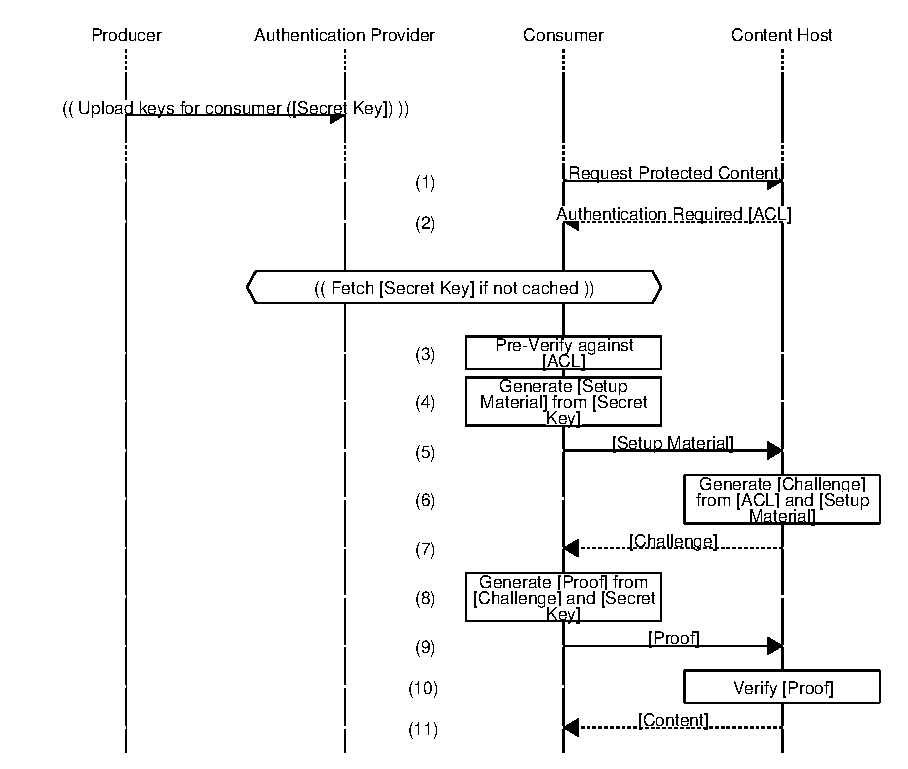
\includegraphics{auth.eps}
\end{figure}

During this protocol, the content host learns precisely that the consumer has
chosen to authenticate to access the piece of content and the consumer learns
the identity of the publisher (listed in the ACL) and how many groups grant them
access.

The consumer always completes the entire protocol. If they choose not to
authenticate, they send cancel at the end. This way, a failure and a cancel are
indistinguishable (see \ref{todo}).

Finally, if the consumer's browser fails to generate the \verb=[Proof]=, it
warns the user. We do this to discourage content hosts from fingerprinting
consumers (see \ref{sub:fingerprinting}).

\subsection{Account Recovery}

\chapter{Related Work and Motivation}

This section discusses related work, existing systems, and the motivation behind
DRACL\@. In short, DRACL provides better usability and privacy guarantees than
any existing fully specified system.

\section{Identity Systems}

The most common access control scheme is to assign one or more unique identities
to all agents and then have all content hosts record which identities have
access to what. We call these identity systems because, while access control
systems can be built on top of them, they don't inherently provide access
control as a feature.

This type of system is inherently bad for privacy because content hosts learn
the identities of who has access to what and, by extension, who knows who. While
this privacy issue sufficiently motivates an alternative design, we have
included this section to give an overview of some common existing systems and to
learn from their shortcomings (in addition to the privacy problem).

\subsection{Site Specific Identity}

The vast majority of content hosts today force users to create site-specific
accounts. This is a poor solution to the access control problem for both users
and content hosts because it adds unnecessary usability and deployability
overhead and introduces security hazards.

% TODO: Cary social network Problems

From a usability standpoint, site-specific accounts force users to create new
accounts and replicate their social networks on every content host they use.
DRACL avoids the first problem by allowing users to create a single account with
a single Authentication Provider for use on multiple content hosts. It avoids
the second problem by handling access control on behalf of the content host.

From a deployability standpoint, site-specific accounts force content hosts to
implement custom account/access control systems and make it harder to attract
new users. DRACL solves the first problem by allowing content hosts to focus on
whether or not an operation should be permitted instead of messing around with
identities.

Site specific accounts are a security hazard because content hosts are
notoriously bad at safely storing credentials and users are notoriously bad at
choosing/remembering safe passwords. Because of this, content hosts often store
user credentials in the clear~\cite{plaintext} and users often reuse passwords
and/or use weak passwords~\cite{ms-passwords}. DRACL reduces these security
hazards by restricting credential checking to APs and reducing the number of
credentials that users have to manage to one (the one they need to authenticate
to their AP).

\subsection{Centralized Identity}

Centralized identity systems, such as those provided by Google and Facebook,
allow users to identify to multiple sites using a set of credentials. These
systems therefore solve all of the security present in site-specific identity
systems as users only have one set of credentials. They also solve the
associated usability problems of having to remember multiple passwords.

While centralized identity systems sometimes increase usability by allowing
users to carry their social networks with them to content hosts (e.g. Facebook),
they don't provide a way to do so while maintaining privacy. That is, for one
user to allow another user to access a resource on a content host, the first
user must identify the second user to the content host. This is a fundamental
problem with identity systems because they operate on the level of identity.
DRACL fixes this problem because it operates on the level of access control.

Again, because these systems operate on identities, they force content hosts to
implement their own access control systems. DRACL, on the other hand, provides
access control out of the box.

Finally, because these systems are centralized, users are forced to choose
between a few ``accepted'' providers and can't run their their own and content
hosts are forced to support whatever identity systems happen to be in vogue at
the time.

\subsection{Decentralized Identity}

Decentralized identity systems such as OpenID~\cite{openid},
Persona~\cite{persona}, and WebID~\cite{webid} allow users to identify to
multiple services using the same credentials but, unlike centralized identity
systems, decentralized identity systems do not force users to choose
between a few ``accepted'' providers. Additionally, in theory, content hosts
should be able to support exactly one decentralized identity system assuming
they eventually converge. While decentralized identity addresses the user choice
concern, it still doesn't address the privacy concern because, again, it
operates on the level of identities.

\section{Access Control Systems}

Unlike identity systems, access control systems directly dictate what operations
a system should and should not permit. Where an identity system answers the
question ``Does PROOF imply that CLIENT is IDENTITY?'', access control systems
answer the question ``Does PROOF imply that CLIENT has PERMISSION?''. In our
case, ``PERMISSION'' is usually ``can access CONTENT''.

\subsection{Centralized Access Control}

Centralized access control systems such as Kerberos~\cite{kerberos} and
LDAP~\cite{ldap} allow services to offload user/group management to third
parties (the access control provider). This solves the some of the  problems noted
in the centralized identity section because the social network is now % TODO
defined in a centralized system (the access control system). However, it makes
the centralization problem much worse because, while content hosts can allow
different users to authenticate with different centralized authentication
services, they cannot allow users to choose their own centralized
access control services without partitioning the social network by access
control service because the access control services don't interoperate.

\subsection{Decentralised Access Control}

Decentralized access control systems such as the one proposed in this document
offer the same benefits as centralized access control systems but without the
drawbacks of being a centralized system. That is, users can freely choose
between providers or run their own. 

Other systems have attempted to address this problem including \cite{attrib}
\cite{privattrib} \cite{drbac} \cite{socnet} and the Kerberos Consortium's User
Managed Access (UMA)~\cite{uma}. Unfortunately, while both \cite{attrib} and
\cite{privattrib} describe cryptographic protocols for privacy preserving
decentralized access control, neither attempt to design an implementable system.
UMA\cite{uma} \cite{drbac} and \cite{socnet} provide a more thorough system
designs (UMA even provides a system specification) but all fail to even address
the question of user privacy.

\subsection{Bearer Credentials}

TODO: Secret URLs, Macaroons (Google, 2014).

\begin{comment}

Macaroons:
Pros:
* Simple
* Easy delegation. This is actually *very nice*.

Cons:
* Easy delegation
* One ``token'' per content.
* No anonymity.
* Policies are not hidden.
\end{comment}

\chapter{Discussion}

Above all, DRACL aims to be practical --- that is, usable in practice, not only
in theory. Additionally, DRACL aims to be secure, privacy preserving, and
developer and user friendly.

\section{Practical}

First, to be practical, we need ``business model.'' In our case, the only
component that needs direct funding are the APs. Some common ways to support
internet services are:

\begin{compactenum}
    \item Charge
    \item Advertise
    \item Sell user information
    \item Accept Donations
    \item Distribute the load
\end{enumerate}

People don't pay for anything they can get for free so 1 is out given that we're
trying to replace a free system. Advertising is intrusive and annoying and we
want DRACL to be as non-intrusive as possible so 2 is out. Selling user
information conflicts with the our privacy goals so 3 is out. Therefore, we are
left with 4 and 5: accept donations and distributing the load.

Therefore, one of the focuses in this protocol is making APs as efficient and
decentralized as possible. We have designed DRACL so that we can run a public AP
on relatively inexpensive hardware and users who don't trust us can run their
own, even on unreliable home connections.

\section{Secure}

DRACL is secure in practice. Being secure in some perfect world where all
software is perfect and bug free isn't practical.

First, only authorized users, the content owner, and the content host are able
to access resources protected by DRACL\@. Specifically, DRACL doesn't allow the AP
to impersonate its users and access their content. A malicious AP may at most
prevent a user from accessing content they should be able to access.

Second, content owners are able recover and secure compromised accounts. User
account compromise is common~\cite{todo} and any system that can't recover from
compromise is dead in the water. We achieve this goal by having APs act as
semi-trusted third parties that certify their content owner's keys with
short-term certificates. Once an AP learns that one of its content owners has
been compromised, it stops signing their keys. The AP then works with the
content owner to transition the content owner to a new set of keys
(authenticating the content owner's identity out-of-band). The details of this
protocol are discussed in section TODO\@. % TODO

Content owners can also efficiently revoke access to content. To facilitate
this, DRACL allows users to be removed from groups without updating every ACL
mentioning the now modified group. Much of the complexity of DRACL stems from
this requirement. Unfortunately, in order to do this efficiently, we sacrificed
some security. Specifically, content published by a content owner before they
remove a consumer from a group will remain accessible to that consumer until
their owner-specific certificate expires. We mitigate this by making
owner-specific certificates short-lived --- they expire on the order of hours.
\todo{There are other ways the content host could learn the consumer's secret is
old...}

Additionally, consumers are discouraged from delegating access. In DRACL, we
chose to do this by making delegation all or nothing. That is, a consumer can
either delegate access to \emph{all} content shared with them by a
\emph{particular content owner} or can delegate access to no content. We would
prefer to make this a true all or nothing by saying that a consumer can only
delegate access to all content of which they are authorized consumers however,
this is impossible without introducing some concept of real-world identity. A
user could simply make one ``identity'' per ``friend''. \todo{Do we really care
about this? Motivate!}

Finally, DRACL cannot interfere with the operation of content hosts. To achieve
this, we guarantee that all DRACL operations performed by the content host will
complete in constant time. As a direct consequence of this, contents host never
initiate network requests on behalf of DRACL\@.

\section{Privacy Preserving}

DRACL preserves the privacy of both content owners and consumers. Preferably,
DRACL would reveal nothing other than whether or not some user should be able to
access some resource. Unfortunately, this goal is impossible to achieve given
our efficiency constraints. However DRACL provides practically optimal privacy
given our performance constraints and some choices we've made when confronted
with unavoidable privacy/security trade-offs.

\begin{description}
\item[Content Host] Content hosts learn the identity of content owners and
  whether or not a given chooses to prove that they have access to a resource.
  Nothing more (except, of course, the content itself).
\item[Consumers] Consumer do not learn which groups any given content owner has
put them in. identity of an ACL's author (content owner) and how many of their
groups them in or which groups are listed in any given ACL\@. However, consumers
do learn precisely how many groups grant them access to a specific piece of
content. Additionally, they learn if a specific content owner has ever granted
them access to some piece of content. Finally, they learn a lower bound on when
the content could have been posted and whether or not the ACL has changed since
the last time they tried to access the content. Unfortunately, this could allow
consumers to to learn with certainty that they have been added or removed from
some set of groups (but not which groups) since they last tried to access the
content.
\item[Authentication Providers] Authentication providers learn nothing but the
  identities of their users and their user's ``popularity''. That is, APs can
  learn the approximate size of a user's social network and how many of these
  friends are active but they \emph{don't} learn what content their users own or
  access, the content hosts they use, or who their friends are.
\item[Collusion] Colluding consumers and content hosts learn nothing more than
  the sum of their knowledge. That is, collusion between any number of content
  hosts and reveals nothing new.
\end{description}

\begin{description}
\item When authenticating, consumers learn only the resource owner and whether
  or not they have access to the resource\footnote{Technically, users learn how
  many groups grant them access to the content.}. Importantly, they learn
  nothing about why they can access the given piece of content (i.e., what groups
  grant them access) or who else might have access to the content.
\item Authentication Providers learn nothing but the identities of their users
  and their ``popularity''. That is, APs can learn the approximate size of a
  user's social network and how many of these friends are active but they
  \emph{don't} learn what content their users own or access, the content hosts
  they use, or who their friends are.
\end{description}


However, we do have some information leaks.

\subsection{Practically Optimal}

We have three privacy leaks that aren't entirely a result of some performance or
privacy trade-off.

First, consumers can learn how many of the groups they are in allow them to
access a resource. That is, given the set of groups a consumer is in,
$\mathbb{U}$, and the set of groups that can access a resource, $\mathbb{R}$,
the consumer can learn the size of the intersection, $|\mathbb{U} \cap
\mathbb{R}|$. This is simply an artifact of the cryptographic protocol we are
using for authentication, not the result of a deliberate efficiency trade-off.

Second, anyone can learn whether or not an ACL has changed since the last time
they accessed a piece of content. In theory, one could randomize challenges so
that they look fresh every time. However, in our opinion, this is more trouble
than it is worth (for security reasons, content hosts present a signed copy of
the ACL along with challenges). Unfortunately, this does allow users to prove
that they have been added to or removed from a group with certainty (by learning
that they have gained/lost access to content without the ACL changing). However,
regardless of what we do, consumers can learn this with high probability (but
not with certainty) by simply assuming that gaining/loosing access to a set of
content is more likely to be the result of being added or removed from a group
than the result of each of those ACLs having been changed in a short period of
time.

Third, consumers can determine a lower bound on when an ACL may have been crated
because we record the ``time'' (technically, a monotonic counter, not the actual
time) the owner last removed a consumer from a group before creating an ACL in
the ACL itself. This allows us to guarantee that all content published
\emph{after} a consumer is removed from a group is never accessible to that
consumer.

%% TODO

\subsection{The Owner Is Public}

In DRACL, a content owner (the author of an ACL) is publicly visible in the ACL
itself. We had four options:

\begin{enumerate}
\item Make the owner public (what DRACL does).
\item Allow users who are authorized consumers of \emph{some} content controlled
  by the owner to learn the identity of the author.
\item Reveal the owner to the content host only.
\item Don't reveal the owner at all.
\end{enumerate}

It's impossible to provide guarantee 4 without sacrificing performance. In
DRACL, we avoid updating individual ACLs (we don't even contact the content
hosts) when the members of a group changes. To do this, we need to use some
additional owner-specific information during authentication to learn if the
consumer is a member of one of the groups listed in the ACL\@. Therefore some
party participating in authentication will learn the owner of the ACL based on
what owner-specific information they end up using. As only the content host and
consumer are directly involved in authentication (for performance and
reliability reasons) one of those two parties will learn who the owner is.

Providing guarantee 3 would either violate our security guarantees and open
content hosts up to denial of service attacks or force the content owner to
contact every affected content host when an ACL changes. As noted above, either
the content host or the consumer needs to learn the owner-specific information.
To prevent the consumer from learning the identity of the owner, we'd either
have to have the content host fetch this information from the owner or have the
owner send this information to the content host. The first option violates our
rule that the content host must never make network requests on behalf of DRACL\@.
As a matter of fact, this would be the worst case scenario: the content host
would be making a network request to a server specified by a client (the content
owner) on behalf of a client (the consumer). On the other hand, having the owner
send the owner-specific information to each content host ahead-of-time would
complicate the content hosts (they would have to listen for ACL updates) and
force the content owners to contact every content host they have ever used when
they change the members of one of their groups.

If we were to provide guarantee 2, DRACL would either scale horribly at the tail
or provide dubious privacy benefit. To access a piece of content, users would
have to linearly search through a list of owner-specific secrets from every user
who has granted them access to some piece of content. For popular users, this
list could be very large. Worse, the size of this list scales based on actions
taken by \emph{other} users, not the consumer in question. We could use a hybrid
approach where ACLs list the content owner's AP but not the content owner. This
way, consumers would only need to remember keys from content owners whose
content they frequently access; they can fetch other keys on-demand from the
listed APs. Unfortunately, the users who care about their privacy the most and
therefore run their own APs will effectively be named in their ACLs because they
are the \emph{only} user of their APs.\todo{I feel like there is a cleaner
  argument here.}


\subsection{Fingerprinting}
\label{sub:fingerprinting}

One problem with any access control scheme is that the content host can
fingerprint users based on what they can and cannot access. The consumer could
make every access request look like it's coming from a new client but this is
infeasible in practice. Instead DRACL allows the user to decide if and when to
authenticate (always for a content host, always for a content owner on a content
host, once, not now, never) and warns users (loudly) when authentication fails.
This way, consumers control what information they give to content hosts and
content hosts can only confirm answers they already suspect.

\subsection{Side Channels}

Finally, they will likely learn about the consumer's browser, IP address, etc.
This is beyond the scope of DRACL system and users that require true anonymity
should use the Tor Browser\cite{todo} or Tails\cite{todo}.

\section{Developer Friendly}

DRACL is easy to deploy on content hosts. In order to be successful, we felt it
necessary to make DRACL easier to deploy than a custom password-based identity
and access control scheme as lack of developer friendliness is commonly
cited~\cite{todo} as a reason OpenID failed.

To achieve this, the DRACL content host server-side library exposes three pure
functions: \verb=is_acl=, \verb=validate_replacement=, and \verb=authenticate=.
\verb=is_acl= simply verifies that an ACL is well formed.
\verb=validate_replacement= takes an old ACL and an ACL transition statement and
returns either the new ACL that should replace the old ACL or an error. Finally,
\verb=authenticate= takes an opaque consumer input and an opaque ACL and returns
one of: \verb=ALLOW=, \verb=DENY(Reason)=, \verb=CONTINUE(OpaqueReply)= where
\verb=OpaqueReply= should be returned to the client as-is. \verb=authenticate=
may also, rarely, return a new ACL with which the content host should should
replace the old one.

\section{User Friendly}

Any security system that gets in users way is doomed from the start. Therefore,
we have designed DRACL to be user friendly and unobtrusive. Specifically:

\begin{enumerate}
  \item Users only have to remember one set of credentials.
  \item Users can take their their social network with them from content host to
    content host without giving up privacy. See the related work section for a
    comparison to Facebook Connect\texttrademark~\cite{todo}
  \item Day to day, DRACL should be unobtrusive and integrate well with content
    hosts.
\end{enumerate}

These last two issues were recently cited~\cite{todo} by Mozilla as one of the
reasons their authentication system, Persona, failed.
\chapter{Design}

TODO:

* Fingerprinting defense: Defend against fingerprinting by punishing content
hosts that try to authenticate consumers against content they *can't* access.

%\chapter{Design}
%
%This section describes the core design and does not include concrete APIs. To
%make this design easy to follow, we'll first map the abstract content owner and
%consumer to concrete entities:
%
%\begin{compactitem}
%    \item The content owner is Penny.
%    \item The consumers are Kevin and Cary.
%\end{compactitem}
%
%Let's also assume that Penny has a stalker, Eve, who wants to see everything she
%(Penny) posts.
%
%Penny has a piece of content she wishes to share with Kevin and Cary using a
%third party service. For this story, let's say she wants to share a photo with
%Kevin and Cary using FoShare as the third party service (the content host).
%However, there's a catch: she doesn't want her stalker, Eve, to see the photo.
%Therefore, along with her photo, she needs to give FoShare some way to
%distinguish ``friend from foe''. We'll call this extra information an ACL (access
%control list). The following sections describe how this can be done.
%
%\section{``Friending''}
%
%Before they can securely share content with each other, Penny, Kevin, Cary, and
%Eve will need some way to securely and identify each other. In this system,
%they'll each use an asymmetric keypair. We will use ECC (elliptic curve
%cryptography) GnuPG keypairs as GnuPG is the de-facto decentralized PKI standard
%and elliptic curve cryptographic schemes produce very short signatures.
%
%Now that they all have unique, provable identities, they need to share these
%identities with each other so that they can talk about each other. They do this
%by exchanging public keys. This is similar to Facebook's process of friending,
%however, unlike Facebook friending, this process doesn't need to be symmetric
%and doesn't inherently give Penny, Kevin, Eve, or Cary access to each other's
%content.  We plan to use services like keybase.io~\cite{keybase} to help with
%the initial key-exchange process.
%
%Now that they can securely identify each other, Penny the content owner could just
%tell FoShare to let Kevin and Cary (the consumers) access her photo
%(identifying them by their public keys). However, this would introduce a privacy
%concern because flicker would be able to learn the identities of the two
%consumers.
%
%Instead, we use an anonymous secure group communication scheme as described in
%\cite{acp2} (based on an Access Control Polynomial (ACP) scheme described in
%\cite{acp}). ACP will allow us to efficiently encrypt a shared secret token with
%multiple secret keys without revealing anything about the secret keys. To be
%able to use ACP, Penny the content owner must first generate secret keys (called
%consumer keys) for every friend with whom she wishes to share content and
%distribute them using her AP (described in the next section).
%
%\subsection{Authentication Provider (AP)}
%
%The Authentication Provider (AP) is simply our way to deal with the fact that
%content owners and consumers aren't always online and, even when they are, they
%are often hidden behind firewalls. The AP will host consumer keys, issue
%certificates of membership (as described in the Groups and Authentication 2.0
%sections), and help both consumers and content owners generate ACLs, manage
%friend lists, authenticate, etc. Additionally, content owner and APs will share
%a ``owner secret'' symmetric key which will be useful in the following sections.
%An AP is to DRACL as an Email Provider is to Email.
%
%For now, content owners must trust their APs to not be actively curious. That
%is, an actively curious AP can access any content owned by a content owner.
%Note, however, that owners do not *report* the content they own to their APs so
%passively curious APs should learn nothing about their content. We may choose to
%limit AP power in the future but doing so will impact usability and performance.
%
%Finally, to make it possible for users to find their friends APs given their
%public keys, each user will list his or her AP in the UID section of his or her
%public PGP key.
%
%\todo{Explain?}
%
%\subsection{Authentication 1.0}
%
%This section describes the basic authentication protocol which we will augment
%in the Authentication 2.0 section.
%
%\subsubsection{Generating An ACL 1.0}
%
%Now that Penny has given Kevin and Cary secret keys, she can create an ACL using
%ACP\@. The ACL has three parts: a challenge, a verifier, and an encrypted
%description. The challenge includes an ACP encrypted random content token, the
%domain of the content host authorized to use this ACL, and the publisher's
%signature. The verifier is just the content token (unencrypted). The description
%is some additional data (encrypted with the publisher secret) that the publisher
%and AP can use to reconstruct the ACL\@. To keep the size of ACL within
%reasonable limits, we will, for now, limit the number of users that can be
%granted access to a particular piece of content to 150. In total, an ACL should
%be under $\unit[4]{KiB}$. In the Groups section, we will discuss methods for
%sharing content with more than 150 consumers.
%
%% NOTE: 128*150 (ACP) + 32*150 (description) + 64*8 (signature) + 128 (content
%% token) + 255*8 (content host id) == 3.3KiB (which gives us room for other stuff).
%
%\begin{figure}[H]
%\begin{minted}{JavaScript}
%{
%    challenge: {
%        data: {
%            acp: ACP(content_token, [
%                Kevin_Penny_Shared_key,
%                Cary_Penny_Shared_Key
%            ]),
%            content_host: "foshare.com"
%        },
%        publisher_signature: ECDSA(Penny_Private_Key, data),
%    },
%    verifier: content_token,
%    description: Encrypted(Penny_publisher_secret, [
%        "Kevin",
%        "Cary"
%    ])
%}
%\end{minted}
%\caption{Example ACL}
%\end{figure}
%
%
%\subsubsection{Authentication 1.0}
%
%Now Kevin learns about the photo (Penny tells him through some side channel,
%e.g.\ email) so he goes to FoShare and asks for it. However, FoShare needs to
%verify that Kevin has permission to access the photo. To do this, FoShare simply
%sends Kevin the challenge, Kevin checks Penny's signature, verifies that that
%the content host listed in the challenge is FoShare to prevent MITM attacks (we
%assume the communication channel is authenticated and encrypted with SSL),
%decrypts the ACP, and returns the content token to FoShare. FoShare then checks
%the response against its copy of the content token, and, if they match, gives
%Kevin access to the content.
%
%Now Eve tries to access the photo. From the ACL, she learns that it was
%published by Penny but that's all she learns because she is unable to decrypt
%the ACP\@. Furthermore, due to the privacy preserving nature of ACP, she is unable
%to learn anything about the members that access to the content. In the end, she
%can't access the photo because she can't recover the content token.
%
%\note{One drawback in this scheme is that, if the content host is
%compromised, all ACLs will need to be recreated. We might be able to use
%asymmetric cryptography to avoid this but that would place an additional burden
%on the content host (the ACLs would larger and the content host would have to
%check an asymmetric signature).}
%
%\subsubsection{Revoking Access 1.0}
%
%To revoke access to a piece of content, Penny simply re-creates the ACL
%associated with the content based on the encrypted description included in the
%original ACL\@.
%
%\subsection{Groups}
%
%While the scheme defined above works, it is missing a key component found in
%most access control schemes: groups. There are two primary usability benefits of
%groups:
%
%\begin{compactenum}
%    \item The ability to repeatedly grant access to a common set of consumers.
%    \item The ability to add/remove a consumer to/from the set of users able to
%        access an entire class of content.
%\end{compactenum}
%
%Unfortunately, we were unable to efficiently achieve the second usability
%benefit while preventing content hosts learning whether or not two users are in
%the same ``group''. Therefore, we have decided to introduce two types of groups:
%``cliques'' and ``organization'' (working names).
%
%\subsubsection{Cliques}
%
%In DRACL, a clique is a grouping of consumers known only to an individual
%publisher. Cliques preserve membership privacy (it's impossible for two members
%of a clique to determine whether or not they are in the same clique) however,
%new clique members will not automatically be granted access to content
%previously made available to the clique and removed clique members will retain
%access to any content made available to the clique before the member was
%removed. In short, cliques provide the first usability benefit but not the
%second.
%
%Implementation wise, cliques are simply an abstraction. When adding a clique to
%an ACL, the simply adds the members of the clique to the ACL\@. This
%trivially maintains the secrecy of clique membership.
%
%\subsubsection{Organization}
%
%An organization is analogous to a traditional POSIX group and can be used in the
%same manner. Unlike clique members, organization members gain access to all
%content ever made available to an organization when they become members and
%lose access if their memberships are revoked.
%
%Organizations are not simply an abstraction. Each organization has a publisher
%unique permanent 64bit ID\@. However, consumers never learn these IDs and content
%hosts only learn about organizations used on their service. % TODO: WORDING
%
%For example, let's say that Penny the publisher now wants to work on a her 6.824
%project with Kevin and Cary. She could just give them access to each piece of
%content individually but that would be cumbersome, especially if she needs to
%add another classmate to the project. So, instead, she creates a ``6.824
%Project'' organization and tells her AP that Kevin and Cary are members of this
%organization.
%
%Finally, we use organizations to circumvent the 150 user limit present in the
%Authentication 1.0 section. Basically, we argue that if a group contains more
%than 150 users, learning that two users are a member of the same group reveals
%relatively little to the content host beyond the fact that they know the
%publisher.
%
%\note{We chose 150 because it is Dunbar's \cite{dunbar} number. While not a hard
%limit on social group sizes, we feel this is a generous upper bound on the
%number of "close friends" a user might have.}
%
%
%
%\subsection{Authentication 2.0}
%
%In this section, we modify the authentication scheme described in Authentication
%1.0 to accommodate organizations. Organization authentication is modeled after
%kerberos~\cite{kerberos}.
%
%\subsubsection{Generating An ACL 2.0}
%
%To accommodate organizations, we include the list of organizations (obscured)
%and a shared secret for verifying membership certificates in the ACL\@.
%
%First, we include an obscured list of organizations by adding a random 16 byte
%nonce and a list of hashed (using MD5) \texttt{(nonce, organization\_id)} tuples
%to the challenge and a list of hashed (again, using MD5)
%\texttt{(content\_host\_name, organization\_ID)} to the verifier. We hash the
%organization IDs in the challenge to prevent non-members from learning anything
%about which organizations have been given access to the piece of content and we
%hash the verifier organization IDs to prevent content hosts from colluding to
%track users across services. We may additionally choose to add decoy (fake)
%organizations to obscure the cardinality. Finally, we add these organization IDs
%to the encrypted description section.
%
%\note{MD5 is sufficiently secure because we don't care about collision
%resistance.}
%
%Next, we generate a shared secret using a well-known epoch published by the  the publisher must also give the content host a
%shared secret. We use derive this secret from the publisher's secret
%(\texttt{SHA256("content host domain"|publisher secret)}) so that content hosts
%must only remember one shared secret per publisher and publishers don't have to
%remember any additional shared secrets beyond the \texttt{publisher secret}.
%
%\note{To make these ACLs ``stand alone,'' content hosts may wish to store this
%shared secret along with each ACL instead of storing it once per publisher.}
%
%
%The following is the example ACL from our story for the project's final report.
%To make this example more general, we have included an additional organization
%(``some other org'').
%
%\begin{figure}[H]
%\begin{minted}{JavaScript}
%{
%    challenge: {
%        data: {
%            nonce: some_nonce,
%            acp: ACP(content_token, []), // Empty
%            organizations: [
%                MD5(824_project|some_nonce),
%                MD5(some_other_org|some_nonce)
%            ],
%            content_host: "foshare.com"
%        },
%        publisher_signature: ECDSA(Penny_Private_Key, data),
%    },
%    verifier: {
%        content_token: content_token,
%        organizations: [
%            MD5(824_project|"foshare.com"),
%            MD5(some_other_org|"foshare.com")
%        ] 
%    },
%    description: Encrypted(Penny_publisher_secret, {
%        organizations: [824_project, some_other_org],
%        acp: []
%    })
%}
%\end{minted}
%\caption{Example ACL 2.0}
%\end{figure}
%
%\subsubsection{Learning About Organizations}
%
%Before being able to prove membership in an organization, consumers need to know
%to which organizations they belong. To learn this, they simply authenticate with
%the publisher's AP and then ask ``which organizations do I belong to?''. The AP
%responds with a list of \texttt{("Organization Name", org\_id)} tuples. In our
%example, Cary would receive the following from Penny's AP:
%\texttt{("6.824 Project", 824\_org)}.
%
%\subsubsection{Authentication 2.0}
%
%Now, to access a piece of content, the consumer can either unwrap the content
%token as described in Authentication 1.0 or prove membership in one of the
%associated organizations. Back to the example, Cary first needs to find the
%intersection between the organizations to which he belongs and the organizations
%to which Penny has granted access (to the final report). To do this, Cary,
%computes \texttt{MD5(nonce|$\text{org}_n$)} for each of Penny's organizations in
%which he is a member. He can then find the intersection between his
%organizations and the organizations listed in the ACL's challenge.
%
%Once the consumer knows the set of intersecting organizations (assuming it's
%non-empty), the browser should ask the user which, if any, organization the user
%would like to use to authenticate. Assuming the consumer decides to authenticate
%as a member of one of the organizations, he or she must then either obtain a
%certificate of membership (for that group, for a specific content host) from the
%publisher's AP or use a cached certificate. Content hosts should generally cache
%knowledge of group memberships.
%
%\note{Browsers should remember this choice and automatically authenticate with
%that organization on this content host in the future.}
%
%A certificate of membership is simply a certificate issued by the publisher's AP
%and symmetrically signed with the secret shared by the content host and the
%publisher (see the Generating an ACL 2.0 section) stating: ``The bearer of this
%certificate is a member of \texttt{MD5(content\_host\_name, organization ID)}. issued:
%\texttt{now}, expires \texttt{some time from now}.'' For example, Cary's certificate
%of membership for ``foshare.com'' would be (symmetric signature omitted):
%
%\begin{figure}[H]
%\begin{minted}{JavaScript}
%{
%    organization: MD5(824_project | "foshare.com"),
%    issued: timestamp,
%    expires: timestamp + 24h,
%}
%\end{minted}
%\caption{Example Certificate of Membership}
%\end{figure}
%
%To obtain a certificate of membership, the consumer authenticates with the
%publisher's AP and then simply asks for one. It's up to the publisher to verify
%that this consumer is a member of specified the organization.
%
%Once the consumer receives the certificate, he or she presents it to the content
%host. The content host checks the signature and, if it verifies and the
%certificate is for an acceptable organization, the content host grants access to
%the content.
%
%\note{Again, assuming a secure channel, there is no risk of a man in the middle
%attack here because this certificate is only valid at the current content host.}
%
%Back to the story, Cary wants to access the final report but is unable to
%decrypt the ACP\@. He then tries to to find an intersection between the
%organizations listed in the ACL and the ones he already knows he is a member of
%(consumers should cache organization memberships when possible to reduce the
%load on APs). As Penny just created this organization, Cary finds no
%intersection so he fetches a new list of organizations from Penny's AP and tries
%again. This time, he learns that the \texttt{824\_project} organization has access
%to the report so he obtains a certificate of membership in the group
%\texttt{824\_project} for the content host FoShare from Penny's AP
%(authenticating with his private key). He then hands this certificate over to
%FoShare which checks the certificate and finally allows Cary to access the
%document.
%
%\subsubsection{Revoking Access 2.0}
%
%Revoking access to consumers listed in the ACP is identical to the 1.0 case.
%Additionally, to revoke access to an entire organization, one simply recreates
%the ACL without that specific organization. However, safely removing a consumer
%from an organization is a bit more difficult.
%
%Simply removing a user from an organization is simple. If Penny wants to kick
%Kevin out of her 6.824 Project group, she can simply tell her AP to issue no
%more certificates of membership to Kevin. Unfortunately, this doesn't revoke
%existing certificates of membership. While they will eventually expire, they
%will remain valid for a period of time. So, while Penny can kick Kevin out
%without any issues, she can't kick Cary out so cleanly because he currently has
%a valid (``zombie'') certificate of membership (see the previous section).
%
%To reduce the impact of ``zombie'' certificates, we introduce a freshness
%constraint. Publishers record the last time they removed a member from an
%organization and, when generating an ACL for a piece of content, they tell the
%content host to not accept any certificates of membership issued before this
%time. This way consumers removed from an organization before the publisher
%gives that organization access to a piece of content will not be able to use
%their ``zombie'' certificates to access that piece of content.
%
%\note{Content hosts must be careful to include and check the issue date in
%cached group memberships information as well.}
%
%With this additional feature, Cary  will be able to continue to access old
%content made available to the organization until his certificate expires but
%will not be able to access new content. 
%
%\section{Implementation Proposal}
%
%So far, we've given a high level description of the system. This section will
%give a high level overview of how we plan to implement this system and the
%components we plan to build. Specifically, we plan to build:
%
%\begin{compactitem}
%\item Plugins for common web servers and frameworks. Specifically, we will
%    target Apache 2.0 and python based frameworks.
%\item A browser extension.
%\item A JavaScript shim library for browsers without the extension.
%    Functionality may be reduced and usability may be impacted on browsers
%    lacking the browser extension.
%\item A reference AP\@.
%\item A reference content host (FoShare).
%\end{compactitem}
%
%\subsection{Browser $\leftrightarrow$ Content-Host API}
%
%We plan on implementing two APIs for content hosts: an HTTP based API and a
%JavaScript based API\@.
%
%The HTTP based API will require browser modification (we will create an
%extension to provide the necessary functionality) but will allow for the
%cleanest integration with servers such as Apache. The HTTP based API will also
%allow us to use this protocol outside of the browser.
%
%We will implement the JavaScript API in both the browser extension and a
%shim library. The in-browser implementation will provide the best user
%experience but we will fall-back to the shim if necessary.
%
%\subsubsection{HTTP}
%
%For now, we do not plan to allow publishers to attach ACLs to content using the
%HTTP protocol. We expect they will do so by, e.g.\ writing custom
%\texttt{.htaccess} files. However, consumers will be able to authenticate over
%HTTP\@.
%
%When a consumer attempts to access content protected by an ACL, the content host
%must return an HTTP 401 Authorization Required response and include a
%\texttt{WWW-Authenticate} header with a URL where the DRACL challenge may be
%found. The consumer should then download the challenge (by issuing a GET
%request), generate a response (see Authentication 2.0), and then repeat the
%original request, this time with an \texttt{Authorization} header containing the
%response to the challenge.
%
%Unfortunately, this scheme requires an additional GET request to fetch the
%challenge because the challenge may be too large to comfortably fit in
%\texttt{WWW-Authenticate} header.
%
%\subsubsection{JavaScript}
%
%The JavaScript API will provide the following methods:
%
%\begin{minted}{JavaScript}
%// Ask a consumer to prove that he or she is authorized to
%// access a piece of content.
%function DRACLAuthenticate(challenge, callback);
%
%// Ask a publisher to create a ACL for the described content.
%// The `contentDescription` argument is a short plain-text
%// description of the content.
%function DRACLCreateACL(contentDescription, callback);
%
%// Ask a publisher to update an ACL\@. The `aclDescription`
%// argument is the description from the ACL itself.
%function DRACLUpdateACL(contentDescription, aclDescription, callback);
%\end{minted}
%
%\subsection{Browser $\leftrightarrow$ Authentication Provider API}
%
%This document will not discuss the specifics of the API for communication
%between consumers, publishers, and APs. While important, the design of this API
%will be driven by implementation needs and is not an API that can be reasonably
%designed in advance. Additionally, this API will only impact browser authors and
%Authentication Providers so, while important, it doesn't have to be elegant.
%
%\subsection{Web Server Plugin APIs}
%
%We will target python based frameworks by building a simple library that
%provides the following two methods:
%
%\begin{minted}{python}
%def create_challenge(ACL):
%    """Returns the challenge field of the ACL\@."""
%    # ...
%
%def check_challenge(ACL, response):
%    """Returns true iff the response is validates."""
%    # ...
%\end{minted}
%
%We will target Apache 2.0 by providing a server plugin and integrating with
%\texttt{.htaccess}.
%
%\section{Discussion}
%
%\subsection{Availability}
%
%This system never requires that the publisher/consumer be online at the same
%time. Both the consumer and producer will be able to use the system from behind
%firewalls.
%
%This system does require that the Authentication Provider be available most of
%the time but can tolerate small windows of down-time. % TODO: Explain?
%
%\subsection{Performance}
%
%\subsubsection{Authentication Provider}
%
%The communication overhead for the Authentication Provider are no worse than
%Kerberos. Consumers will re-use their secret keys so they will only have to
%communicate with Authentication Providers to retrieve organization membership
%certificates. As this organization certificate system is modeled after Kerberos,
%its performance characteristics should be similar.
%
%Producers only need to contact their Authentication Providers when modifying their
%friend-list so the \emph{overhead} should be zero. That is, managing a
%friend-list always requires communication and DRACL doesn't add any additional
%communication requirements.
%
%The storage overheads per user are:
%
%\begin{compactitem}
%\item 1 Elliptic Curve Key Key Pair ($\unit[256]{bits}$)
%\item 1 Publisher Secret ($\unit[256]{bits}$)
%\item Two shared secrets per friend (assuming bi-directional friendship)
%    ($\unit[128]{bits}$ each, estimated 300 friends per user = $\unit[9.36]{KiB}$)
%    % TODO: shared secret too small?
%\item Organization IDs ($\unit[64]{bits}$ each, estimated 10 per user = $\unit[70]{KiB}$).
%\end{compactitem}
%
%Conservatively, no Authentication Provider should have to store more than
%$\unit[100]{KiB}$ (including miscellaneous metadata) per user.
%
%The cryptographic overhead is minimal. The Authentication Provider must verify
%an ECDSA signature to authenticate consumers once per ``session'' but can cache
%a user's identity using a cookie (TBD). The AP must also compute one symmetric
%signature per organization membership certificate issued but this overhead will
%quickly be dwarfed by whatever crypto is used to secure the communication
%channel.
%
%\subsubsection{Content Host}
%
%Facebook users publish 2.5 Million pieces of content per day on average in 2012
%(about $\unit[500]{TB}$ of data)~\cite{fbnum}. This is about $\unit[195]{KiB}$
%per piece of content so a $\unit[4]{KiB}$ overhead won't hurt too much ($2\%$
%overhead).
%
%On the other hand, tweets have an upper limit of 140 bytes so a $\unit[4]{KiB}$
%overhead means that issuing per-tweet ACL's will lead to a $2826\%$ minimum
%overhead. This will bump Twitter's data storage requirements up from
%$\unit[65]{GiB}$ per day to $\unit[2]{TiB}$ per day (based on a 500 million
%tweets per day claim made by twitter\cite{twitter}. Unfortunately, ECDSA
%signatures themselves take 64 bytes so we're stuck with a $50\%$ overhead per
%tweet from the signature alone (and ECDSA signatures are some of the shortest
%around \cite{todo}). Therefore, I feel that per-tweet ACLs are simply
%infeasible.
%
%Currently, all of these storage overheads translate directly into communication
%overheads. We could support sending partial ACL challenges however, this just
%isn't worth the trouble. Even when using ACL's large enough to support 1200
%independent ACP entries (8 times the current size), batching 20 resource
%requests together to reduce the effects of latency, and splitting ACL's 16 ways,
%ACL splitting only yields a 6x speedup (assuming $\unit[50]{ms}$ network
%latencies and the world-wide bandwidth average of
%$\unit[3.6]{Mbps}$~\cite{akamai}). Once the bandwidth is bumped up to the FCC's
%broadband definition ($\unit[25]{Mbps}$)~\cite{fcc} the speedup drops to 1.5x.
%
%Again, the cryptographic overhead is minimal. The content host may have to
%verify a single symmetric signature per piece of content accessed (the
%pathological worst case scenario where each piece of content has been published
%to a different organization). However, this overhead should again be dwarfed by
%the overhead of the crypto used to secure the communication channel.
%
%\subsection{Security Concerns}
%
%\subsubsection{Access Delegation}
%
%The primary security issue in this system is access delegation. That is,
%consumers can delegate their access to content either intentionally or
%unintentionally (due to a security breach).
%
%A consumer can indefinitely delegate (give away) access to all content shared
%with him or her by a single friend by giving away his or her shared secret. We
%hope that giving away access to everything will be enough to prevent them from
%doing so willingly.
%
%A consumer can temporarily give another user access to resources published to an
%organization by giving away his or her membership certificate. Fortunately, this
%fine-grained delegation is only possible for short periods of time because these
%certificates expire.
%
%The biggest concern is what happens if an attacker steals a user's credentials.
%Currently, there is nothing we can do to recover.
%
%\subsection{Privacy}
%
%The content host can map users to host-specific organization identifiers and
%colluding users can determine if they are in the same organization. However, for
%small groups (Cliques), group membership is completely hidden.
%
%\subsection{Usability}
%
%This protocol should be very easy for content hosts to implement. From the
%content-host's perspective, the authentication mechanism is stateless.
%Furthermore, the content-host never needs to contact the Authentication Agent
%when authenticating which means that the server-side DRACL code can be
%sandboxed.

% TODO

%* Handling Security Compromises
%
%  - Relying Agent (replacing compromised ACLs)
%
%  - Consumers
%
%  - Publishers
%
%* Remove users from groups.
%
%* Prevent group members from permanently delegating privileges.
%
%* Safely using credentials on untrusted hardware.
%
%* Syncing and Backing up credentials between machines.
%
%* Avoid creating one-off groups (multiple groups in an ACL).
%
%* A distributed key distribution system.
%
%* Make it possible to decrypt an {encrypted token} without trying every group
%  known key.
%
%* Prevent MITM\@. Currently, Kevin must trust that FoShare isn't actually Eve in
%  disguise.
%
%
%# Key distribution service.

\bibliographystyle{acm}
\bibliography{thesis}

\end{document}
% vim: set foldmethod=marker: %
